\section{Package Overview}
%The following diagram shows the most important packages of the \salespoint and their dependencies. These packages are detailed in the chapters below.
Figure \ref{package_overview} depicts the package structure of \salespoint{}.
\begin{figure}[ht]
	\centering
  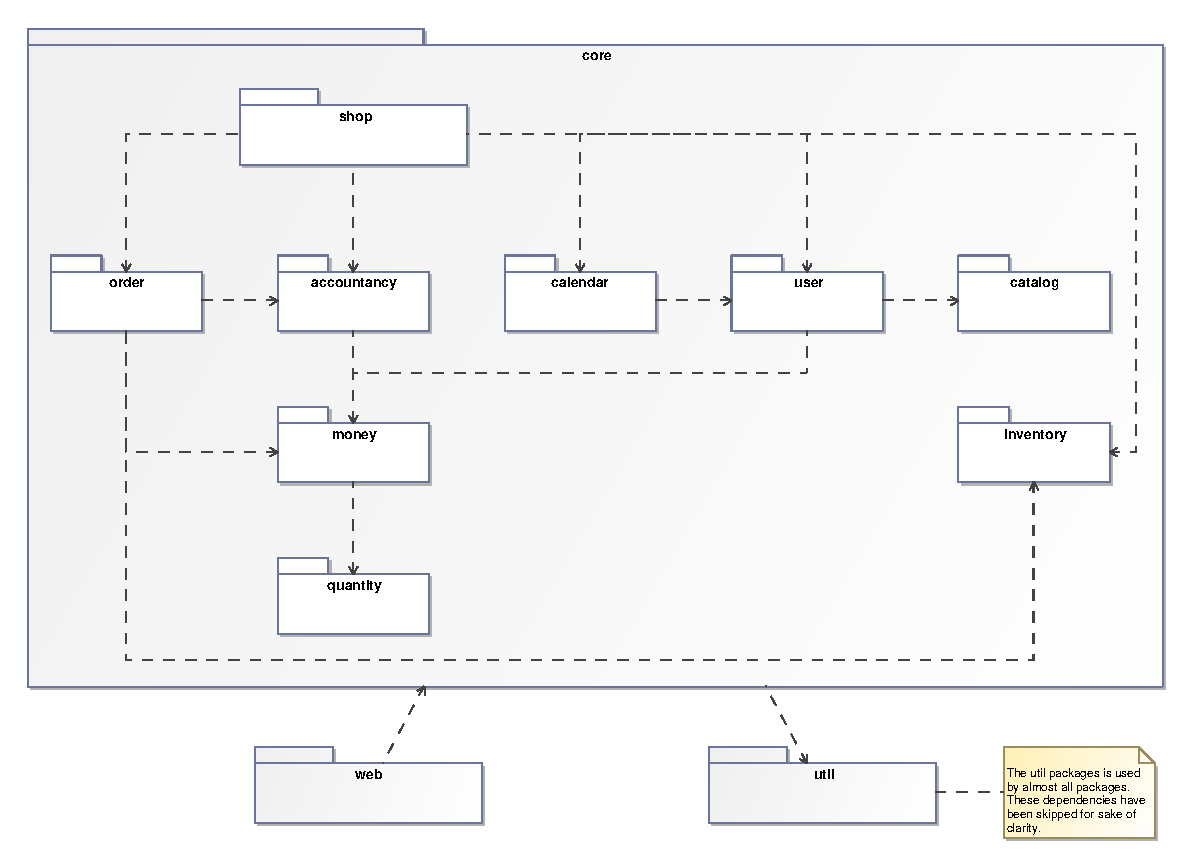
\includegraphics[width=1.0\textwidth]{images/Package_Overview.eps}
	\label{package_overview}
	\caption{Package Overview}
\end{figure}


Objects which need to be persisted, to safe the current state of an application are called persistence entities.
Usually, a persistence entity is a \textit{Plain Old Java Object} (POJO).
Every persistency entities class is an implementation of a corresponding Java interface.
Each persistence entity has a manager class, which in turn is an implementation of a manager interface.
The specific manager implementations in \salespoint{} facilitate persisting the objects to a database.

\salespoint{} strongly advocates the \textit{programming against interfaces} programming style.
Although, creating an interface for almost every class violates the \textit{KISS} principle, the developers deemed programming against interfaces necessary because \salespoint{} is intrinsically tied to JPA.
Using interfaces allowed us to cleanly define the behaviour of an object, without relying on a specific implementation.
Thus it is possible to implement every persistence entity and manager class in \salespoint{} to not be persistent, but, for example, as collection-based.

\salespoint{} is designed to be developer-friendly.
A crucial part of its easy-to-use feel is the consistency in interfaces, persistence entities and managers across the framework, including, but not limited to naming of methods and behaviour of managers.

